\documentclass[journal, spanish]{IEEEtran}

% *** CITATION PACKAGES ***
\usepackage[style=ieee]{biblatex} 
\bibliography{Bibliography/example-bib} %your file created using JabRef
\usepackage{hyperref}
\usepackage{amssymb}
\usepackage{amsfonts}
\usepackage{pdfpages}
\usepackage[electronic]{ifsym}
\usepackage[siunitx, RPvoltages]{circuitikz}
\usepackage{tikz}
\usetikzlibrary[cd]
\usetikzlibrary{shapes,arrows}
\usepackage{ifthen}
\usepackage{listings}
\usepackage{minted}
\usepackage{verbatim}
\usepackage{schemabloc}
\usepackage{flowchart}

\ctikzset{
    amplifiers/fill=cyan,
    %sources/fill=green,
    diodes/fill=green,
    resistors/fill=violet,
}
% TIENG VIET THI UNCOMMENT DONG BEN DUOI
\usepackage[spanish]{babel}
\usepackage[utf8]{inputenc}
\usepackage{csquotes}
\usepackage{amsmath}
% *** MATH PACKAGES ***
\usepackage{amsmath}
\usepackage{multirow}
% *** PDF, URL AND HYPERLINK PACKAGES ***
\usepackage{url}
\hypersetup{
    linkcolor=blue,
    urlcolor=red,
}
% correct bad hyphenation here
\hyphenation{op-tical net-works semi-conduc-tor}
\usepackage{graphicx}  %needed to include png, eps figures
\usepackage{float}  % used to fix location of images i.e.\begin{figure}[H]

\raggedbottom

\begin{document}

% paper title
\title{Plantilla IEEE para plataformas \LaTeX \\
\small{Actividad de aprendizaje: Diseñar una plantilla con extensión .tex}}

% author names 
\author{Author1 name - correo@correo.edu.co \\Author2 name - correo1@correo.edu.co \\Author3 name - correo3@correo.edu.co \\Author4 name - correo4@correo.edu.co}
% <-this % stops a space
        
% The report headers
\markboth{Bogotá Colombia - \today}%do not delete next lines
{Shell \MakeLowercase{\textit{et al.}}: Bare Demo of IEEEtran.cls for IEEE Journals}

% make the title area
\maketitle

% As a general rule, do not put math, special symbols or citations
% in the abstract or keywords.
\begin{abstract} 
En el siguiente documento se pretende crear una plantilla IEEE LaTeX, en el cuál, también seŕa una guía de introduccioń a latex a dobble columna.
\end{abstract} 

\begin{IEEEkeywords}
iEEE, LaTeX, bib, GitHub.\\
\end{IEEEkeywords}

\textbf{Reflexión:} Es indispensable al momento de presentar un informe de laboratorio, sustentación de proyecto de aula o tésis de grado , en el cual se requiera  orden, el anexo de imágenes, tablas, diagramas, referenciar autores y la inserción de ecuaciones que, en ciertos sofware se realiza de forma aleatoria y/o no posee los carácteres especializados para plasmar: Una ecuación matemática o física, código de una consola de programación o fórmulas químicas, en cualquier caso, LaTex será una herramienta facilitadora de su trabajo. Recuerde que  \textit{\textbf{“Somos lo que hacemos reiteradamente. La excelencia, por tanto, no es un acto, sino un hábito” \textsc{- Arístóteles.}}} \\¡¡Bienvenido a \LaTeX!!


\section{Introducción}
%\IEEEPARstart{D}{escribe:} 
Para este documento se tiene como propósito profundizar los conceptos y conocimientos en el manejo de LaTex, asi mismo promover la escritura académica y científica.
\subsection{\bf Software utilizado}
\begin{itemize}
    \item LATeX.
    \item Git y GitHub.
\end{itemize}
\subsection{\bf GLOSARIO}
\begin{itemize}
    \item {\bf LaTeX:} which is pronounced «Lah-tech» or «Lay-tech» (to rhyme with «blech» or «Bertolt Brecht»), is a document preparation system for high-quality typesetting. It is most often used for medium-to-large technical or scientific documents but it can be used for almost any form of publishing.\cite{noauthor_introduction_nodate}
    \item {\bf IEEE:} The Institute of Electrical and Electronics Engineers (IEEE) is a professional association for electronic engineering and electrical engineering (and associated disciplines).\cite{noauthor_institute_2021}
    \item {\bf GitHub:} is a for-profit company that offers a cloud-based Git repository hosting service. Essentially, it makes it a lot easier for individuals and teams to use Git for version control and collaboration.\cite{noauthor_what_nodate}
\end{itemize}
\section{Análisis}
Se debe tener en cuenta que \LaTeX es un tipo de lenguaje muy similar a XML, es decir cada "item" nuevo que se abra, cada instrucción nueva debe tener su final, su cierre de ciclo. También se a agregado una carpeta llamada Images el cual contendra las imagenes utilizadas en el archivo, también se a agregado un archivo llamado example-bib.bib el cual es donde estarán todas las referencias, citas, para agregar a la bibliografía, el contenido de este archivo es de estructura .bib, en nuestro caso utilizaremos \textit{Zotero} para agregar referencias fácilmente al informe.\\
Si desea tener acceso al código fuente .tex ingrese a \url{https://github.com/Amigs/IEEE_template__LaTex}.

\section{Procedimiento}
Con el fin de hacer de esta plantilla una guía para iniciar con Latex en el ámbito IEEE, en esta sección procederemos a incluir imagenes, tablas, lineas de código, citas, y así poder darle un aventón al mundo de las posiblidades que puedes hacer con \textbf{\LaTeX}.
\subsection{\textsc{Imágenes y diagramas.}}
Para incluir imagenes se sigue un estandar muy básico de aplicar, lo único a tener en cuenta es el tamaño de estas y como queremos que se vizualice en el documento.\\

\noindent En la figura \ref{fig:led_Frit} podemos ver que está centrada y con un tamaño predefinido:
\begin{figure}[H]%[!ht]
    \begin {center}
        
\includegraphics[width=5.8cm, height=5.5cm]{Images/Latex.jpeg}
        \caption{Manejo de imágenes en LaTeX.}
        \label{fig:led_Frit}
    \end {center}
\end{figure}

\noindent También podemos colocar la imagen con inclinación como se puede apreciar en la figura \ref{fig:images}:
\begin{figure}[H]%[!ht]
    \centering
    \caption{Inclinando imágenes en LaTeX.}
    
\includegraphics[width=5.6cm, height=4.45cm, angle=180]{Images/Latex.jpeg}
    \label{fig:images}
\end{figure}

\noindent Haciendo uso del package circuitikz y sus complementos, Latex también nos ofrece la capacidad de crear circuitos electrónicos apartir de línea de código, acontinuación se muestran algunos ejemplos:\\

\begin{center}
    \begin{circuitikz}[american]
        \draw (0,0) to[isource, l=$I_o$,v=$V_0$] (0,3) -- (2,3)to[R=$R$] (2,0) -- (0,0);
    \end{circuitikz}
    \begin{circuitikz}[american]
        \draw (0,0) to[battery,v=$V_0$] (0,3) -- (2,3)to[C=$C$] (2,0) -- (0,0);
    \end{circuitikz} 
\end{center}
\begin{center}
    \begin{circuitikz}[american]
        \draw (0,0) to[isource, l=$I_0$] (0,3) -- (2,3) to[R=$R$,v=$V_0$] (2,0) -- (0,0);
        \draw (2,3) -- (4,3) to[L=$L$] (4,0) -- (2,0);
    \end{circuitikz}
\end{center}
\begin{center}
    \begin{circuitikz}[american]
        \draw (0,0) to[isource, l=$I_0$] (0,3) to[short, -*, i=$I_0$] (2,3)
            to[R=$R_1$, i>_=$i_1$] (2,0) -- (0,0);
        \draw (2,3) -- (4,3) to[R=$R_2$, i>_=$i_2$] (4,0) to[short, -*] (2,0);
    \end{circuitikz}
\end{center}
\begin{center}
    \begin{circuitikz} 
        \draw[black](0,2) node[and port] (myand1) {\tiny$AND_1$}
        (0,0) node[and port] (myand2) {\tiny$AND_2$}
        (2,1) node[xnor port] (myxnor) {\tiny$xnor$}
        (myand1.out) -| (myxnor.in 1)
        (myand2.out) -| (myxnor.in 2);
        \node [left, font=\small]
        at (myand1.in 1) {$a$};
        \node [left, font=\small]
        at (myand1.in 2) {$b$};
        \node [left, font=\small]
        at (myand2.in 1) {$c$};
        \node [left, font=\small]
        at (myand2.in 2) {$d$};
        \node [right, font=\small]
        at (myxnor.out) {$Out$};
    \end{circuitikz}
    \begin{circuitikz} \draw 
    (0,0) node[op amp] (opamp) {}
    (opamp.+) node[left] {$v_+$}
    (opamp.-) node[left] {$v_-$}
    (opamp.out) node[right] {$v_o$}
    (opamp.down) node[ground] {}
    (opamp.up) ++ (0,.5) node[above] {\SI{12}{\volt}} -- (opamp.up);
    \end{circuitikz}
\end{center}
\begin{center}
    \begin{circuitikz}
        \ctikzset{multipoles/thickness=2}
        \ctikzset{multipoles/external pins thickness=2}
        \draw (0,0) node[dipchip,
            num pins=12,
            hide numbers,
            external pins width=0.2,
            external pad fraction=6 ](C){$\small\mu$};
        \draw (C.pin 8) -- ++(0.4,0) to[switch] ++(1.5,0) node[left]{} ++(0.35,0) node[]{$5V$};
        \draw (C.pin 7) -- ++(0.5,0) to[D] ++(0,-1) node[ground]{};
            \node [right, font=\tiny]
            at (C.bpin 5) {VB};
            \node [right, font=\tiny]
            at (C.bpin 1) {C13};
            \node [right, font=\tiny]
            at (C.bpin 3) {C14};
            \node [left, font=\tiny]
            at (C.bpin 8) {G};
            \node [left, font=\tiny]
            at (C.bpin 7) {out};
    \end{circuitikz}
\end{center}
Los colores que presenta el diodo y el OPAM se establecieron al principio del documento dentro de la estructura: ctikzset.

\noindent Para finalizar está sección también se muestra como realizar diagramas para sistemas de control a partir de código ofrecidos por package en \LaTeX.

\begin{center}
    \begin{tikzpicture}
        \begin{small}
            \sbEntree{E}
            \sbComp[1.5]{comp}{E}
            \sbRelier{E}{comp}
            \sbBloc[1.5]{B}{$\dfrac{K}{1+p+p^2}$}{comp}
            \sbRelier{comp}{B}
            \sbSortie{S}{B}
            \sbRelier{B}{S}
            \sbRenvoi{B-S}{comp}{}
        \end{small}
    \end{tikzpicture}
\end{center}
\begin{center}
    \begin{tikzpicture}
    \sbEntree{E1}
    \sbBloc[3]{Bloc1}{$H1$}{E1}
    \sbRelier[$E(p)$]{E1}{Bloc1}
    \sbBloc[3]{Bloc2}{$H2$}{Bloc1}
    \sbRelier[]{Bloc1}{Bloc2}\sbSortie[3]{S1}{Bloc2}
    \sbRelier[$S(p)$]{Bloc2}{S1}
    \end{tikzpicture}
\end{center}
\begin{center}
    \begin{tikzpicture}
        \begin{small}
        \sbEntree{E}
        \sbBoucleSeule[3]{E}{A/$A_1(p)$,B/F(p),D/$D(p)$}{S}
        \end{small}
    \end{tikzpicture}
\end{center}
\begin{center}
    \begin{tikzpicture}
        \begin{small}
        \sbEntree{U}
        \sbBoucleRetour[3]{U}{A/$Control$,B/$Sistema$,D/$Actuador$}{G/$Sensor$}
        \node[above of=CompU-A,node distance=0.5em] {$\varepsilon(p)$};
        \node[above of=A-B,node distance=0.5em]{$u(p)$};
        \node[above of=U,node distance=0.8em]{$In$};
        \sbSortie[3]{V2}{D}\sbRelier[$Out$]{D}{V2}
        \end{small}
    \end{tikzpicture}
\end{center}

\subsection{TABLAS}
\noindent
En está sección se abordará de manerá rápida como incluir tablas y trabajar con ellas.

 \begin{table}[h]
   \centering
   \begin{tabular}{ c |  c | c }
    \textbf{\textit{a}} &    & \\ \hline
    & \textbf{\textit{b}} & \\ \hline
    &  & \textbf{\textit{x}} \\ \hline
    &    &  \\
   \end{tabular}%
 \quad$ \dashrightarrow $\quad
    \begin{tabular}{ c |  c | c }
     \textbf{\textit{a}} &\textbf{\textit{ c}}  & \\ \hline
     \textbf{\textit{d}} & \textbf{\textit{b}}  & \\ \hline
     \textbf{\textit{e}} & \textbf{\textit{f}}  & \\ \hline
     &    &  \\
    \end{tabular}
    \caption{Dos tablas en misma línea}
 \end{table}
 \begin{center}
    \begin{tabular}{llcr}
    pepino & tomate & berenjena & rábano \\
    manzana & naranja & fresa & pera \\
    papa & cubíos & zanahoría & fríjol \\
    Banano & sandía & uva & limón \\
    ajo & cebolla & lechuga & Espinaca \\
    piña & melocotón & coco & frambuesa \\\\\\
    \end{tabular}
\end{center}

\noindent Las tablas en LaTeX tiene muchas variantes en cuanto a su uso, todo depende de como la desees ver tú, otra forma típica, se puede ver en el cuadro \ref{tabla:final}:
\begin{table}[htb]
    \centering
    \begin{tabular}{|l|l|l|l|}
        \hline
        & \multicolumn{3}{c|}{\bf Europa} \\
        \cline{2-4}
        & \bf Ciudad & \bf Río & \bf Símbolo\\ \hline 
        \multirow{3}{1cm}{\bf España} & Madrid & Manzanares & Cibeles\\ \cline{2-4}
        & Sevilla & Guadalquivir & Giralda\\ \cline{2-4}
        & Zaragoza & Ebro & Pilar\\ \cline{1-4}
        \bf Francia & París & Sena & Torre Eiffel\\ \cline{1-4}
        \multirow{2}{1cm}{\bf Italia} & Roma & Tíber & San Pedro\\ \cline{2-4}
        & Milán & \multicolumn{1}{c|}{-} & Duomo\\ \cline{1-4}
    \end{tabular}
\caption{Table so pretty}
\label{tabla:final}
\end{table}
\begin{table}[htb]
    \centering
    \begin{tabular}{|l|r|r|}
    \hline
        & \multicolumn{2}{c|}{Distancia al sol} \\
    Planeta   &  \multicolumn{2}{c|}{(millones km)} \\ \cline{2-3}
    & Máxima  &   Mínima   \\ \hline
    Mercurio  & 69.4  & 46.8  \\
    Venus     & 109.0 & 107.6 \\
    Tierra    & 152.6 & 147.4 \\ \hline
    \end{tabular}
    \caption{Jugando con las columnas}
\end{table}
\subsection{ECUACIONES Y SÍMBOLOS}
\noindent LaTeX se caracteriza por su podera escritura de ecuaciones y símbolos matemáticos, acontinuación se plasmaran algunos ejemplos, los cules serán de gran utilidad.
\begin{gather}
    \Delta_x \\ \Delta_y\\
    130x+ 4z = y+ 2\\
    43y+ 57z = 20x+ 99\\
    43y+ 57z = 20x+ 33
\end{gather}

$$\dot{x},\ddot{x}$$
$$ x_{ij},x^{2} $$
$$\sum, \sum_{i=1}^{20}{5x}$$
$$5\pm{5cm}$$
$$5\cong{5cm}$$
$$\iint\limits_0, \iiint\limits, \iiiint$$
$$\nabla{f}, \frac{dx}{dy}$$
$$\lim_{x\to 0}, \underset{x\to 0}{\lim}$$

\begin{subequations}
    \begin{equation}
        5x+2y = 2z+3 \label{eq1}
    \end{equation}
    \begin{equation}
        \boxed {x = \frac{-2y+2z+3}{5}} \label{eq2}
    \end{equation}
\end{subequations}

\noindent Es muy importante mencionar el uso de referncias durante el texto, bien pude ser referenciando una imagen, un diagrama, una tabla, una ecuación, lo importante es la palabra reservada $label$ el cual sera de guía de referncia. \\

\noindent La solución a la ecuación de la figura \ref{fig:led_Frit} se puede ver en expresada en las ecuaciones \eqref{eq1} y \eqref{eq2} sucesivamente.

\begin{equation*}
    \mbox{Updated value}\quad x= x^\mathrm{low} + yd \enspace.
\end{equation*}

\begin{equation}
    \mbox{Updated value}\quad x= x^\mathrm{low} + yd \enspace.    
\end{equation}
\noindent Evaluar la velocidad dos segundos después de haber inciado el cronómetro:
\begin{equation*}
    \begin{split}
        f(x) &= x^3 + 2x^2 - 5x + 10\\
        f(2) &= (2)^3 + 2(2)^2 - 5(2) + 10\\
        &= 16
    \end{split}
\end{equation*}

\noindent También distintos tipos de matrices.

\begin{equation*}
    \begin{pmatrix} x_1 \\ x_2+7 \end{pmatrix}
\end{equation*}

\begin{equation*}
    \begin{bmatrix} 1-y & 0 \\ 0 & 1-y \end{bmatrix}
\end{equation*} 

\begin{equation*}
    \left[ \begin{array}{rrr}
    33 & 0 & 375\\
    289 & 470 & 8\\
    7 & 14 & 67
    \end{array} \right]
\end{equation*}

\begin{equation*}
    \left[\begin{array}{cccc}
    k_{11} & k_{12} & \ldots & k_{1n}\\
    k_{21} & k_{22} & \ldots & k_{2n}\\
    \hdotsfor{4}\\
    k_{n1} & k_{n2} & \ldots & k_{nn}
    \end{array}\right]
    %
    \left\{\begin{array}{c}
    x_1\\x_2\\ \hdotsfor{1}\\x_n
    \end{array}\right\} =
    %
    \left\{\begin{array}{l}
    f_1+a\\f_2\\ \hdotsfor{1}\\f_n+c
    \end{array}\right\}
\end{equation*}
\subsection{BASH Y SCRIPTS}
Para finalizar el documento se presenta dos maneras distintas para escribir tu código dentro del documento, se debe encuenta que si el código es muy exteso, será preferible incluirlo en la sección de anexos, el cual se encuentra en la parte final del documento. \\

\noindent En el siguiente código se realiaz un  hola mundo!
\begin{lstlisting}[language=C]
#include <stdio.h>
int main(int argc, char* argv[]) {
puts("Hola mundo!");
}
\end{lstlisting}
\begin{minted}{c}
#include <stdio.h>
int main(int argc, char* argv[]) {
puts("Hola mundo!");
}
\end{minted}
En ejemplo anterior se configuro para programación en lenguaje C, pero también es útil para los demas lenguajes de programación como por ejemplo:
\begin{itemize}
    \item Python.
    \item Java.
    \item Ruby.
\end{itemize}
\section{Conclusiones}
\begin{itemize}
    \item Se elaboro con éxito la plantilla, con el fin de promover el aprendizaje e impulsar el uso correcto de la escritura académica.
    \item En la actualidad  es de vital importancia saber escribir bien, y con herramientas como Latex podemos llevar a cabo esa tarea a un nivel académico profesional.
    \item Utilizar paquetes puede llevar nuestra expreiencia un paso más allá, además es correcto evitar errores en la creación del documento.
\end{itemize}
\printbibliography[title={\section{Referencias}}]
\clearpage
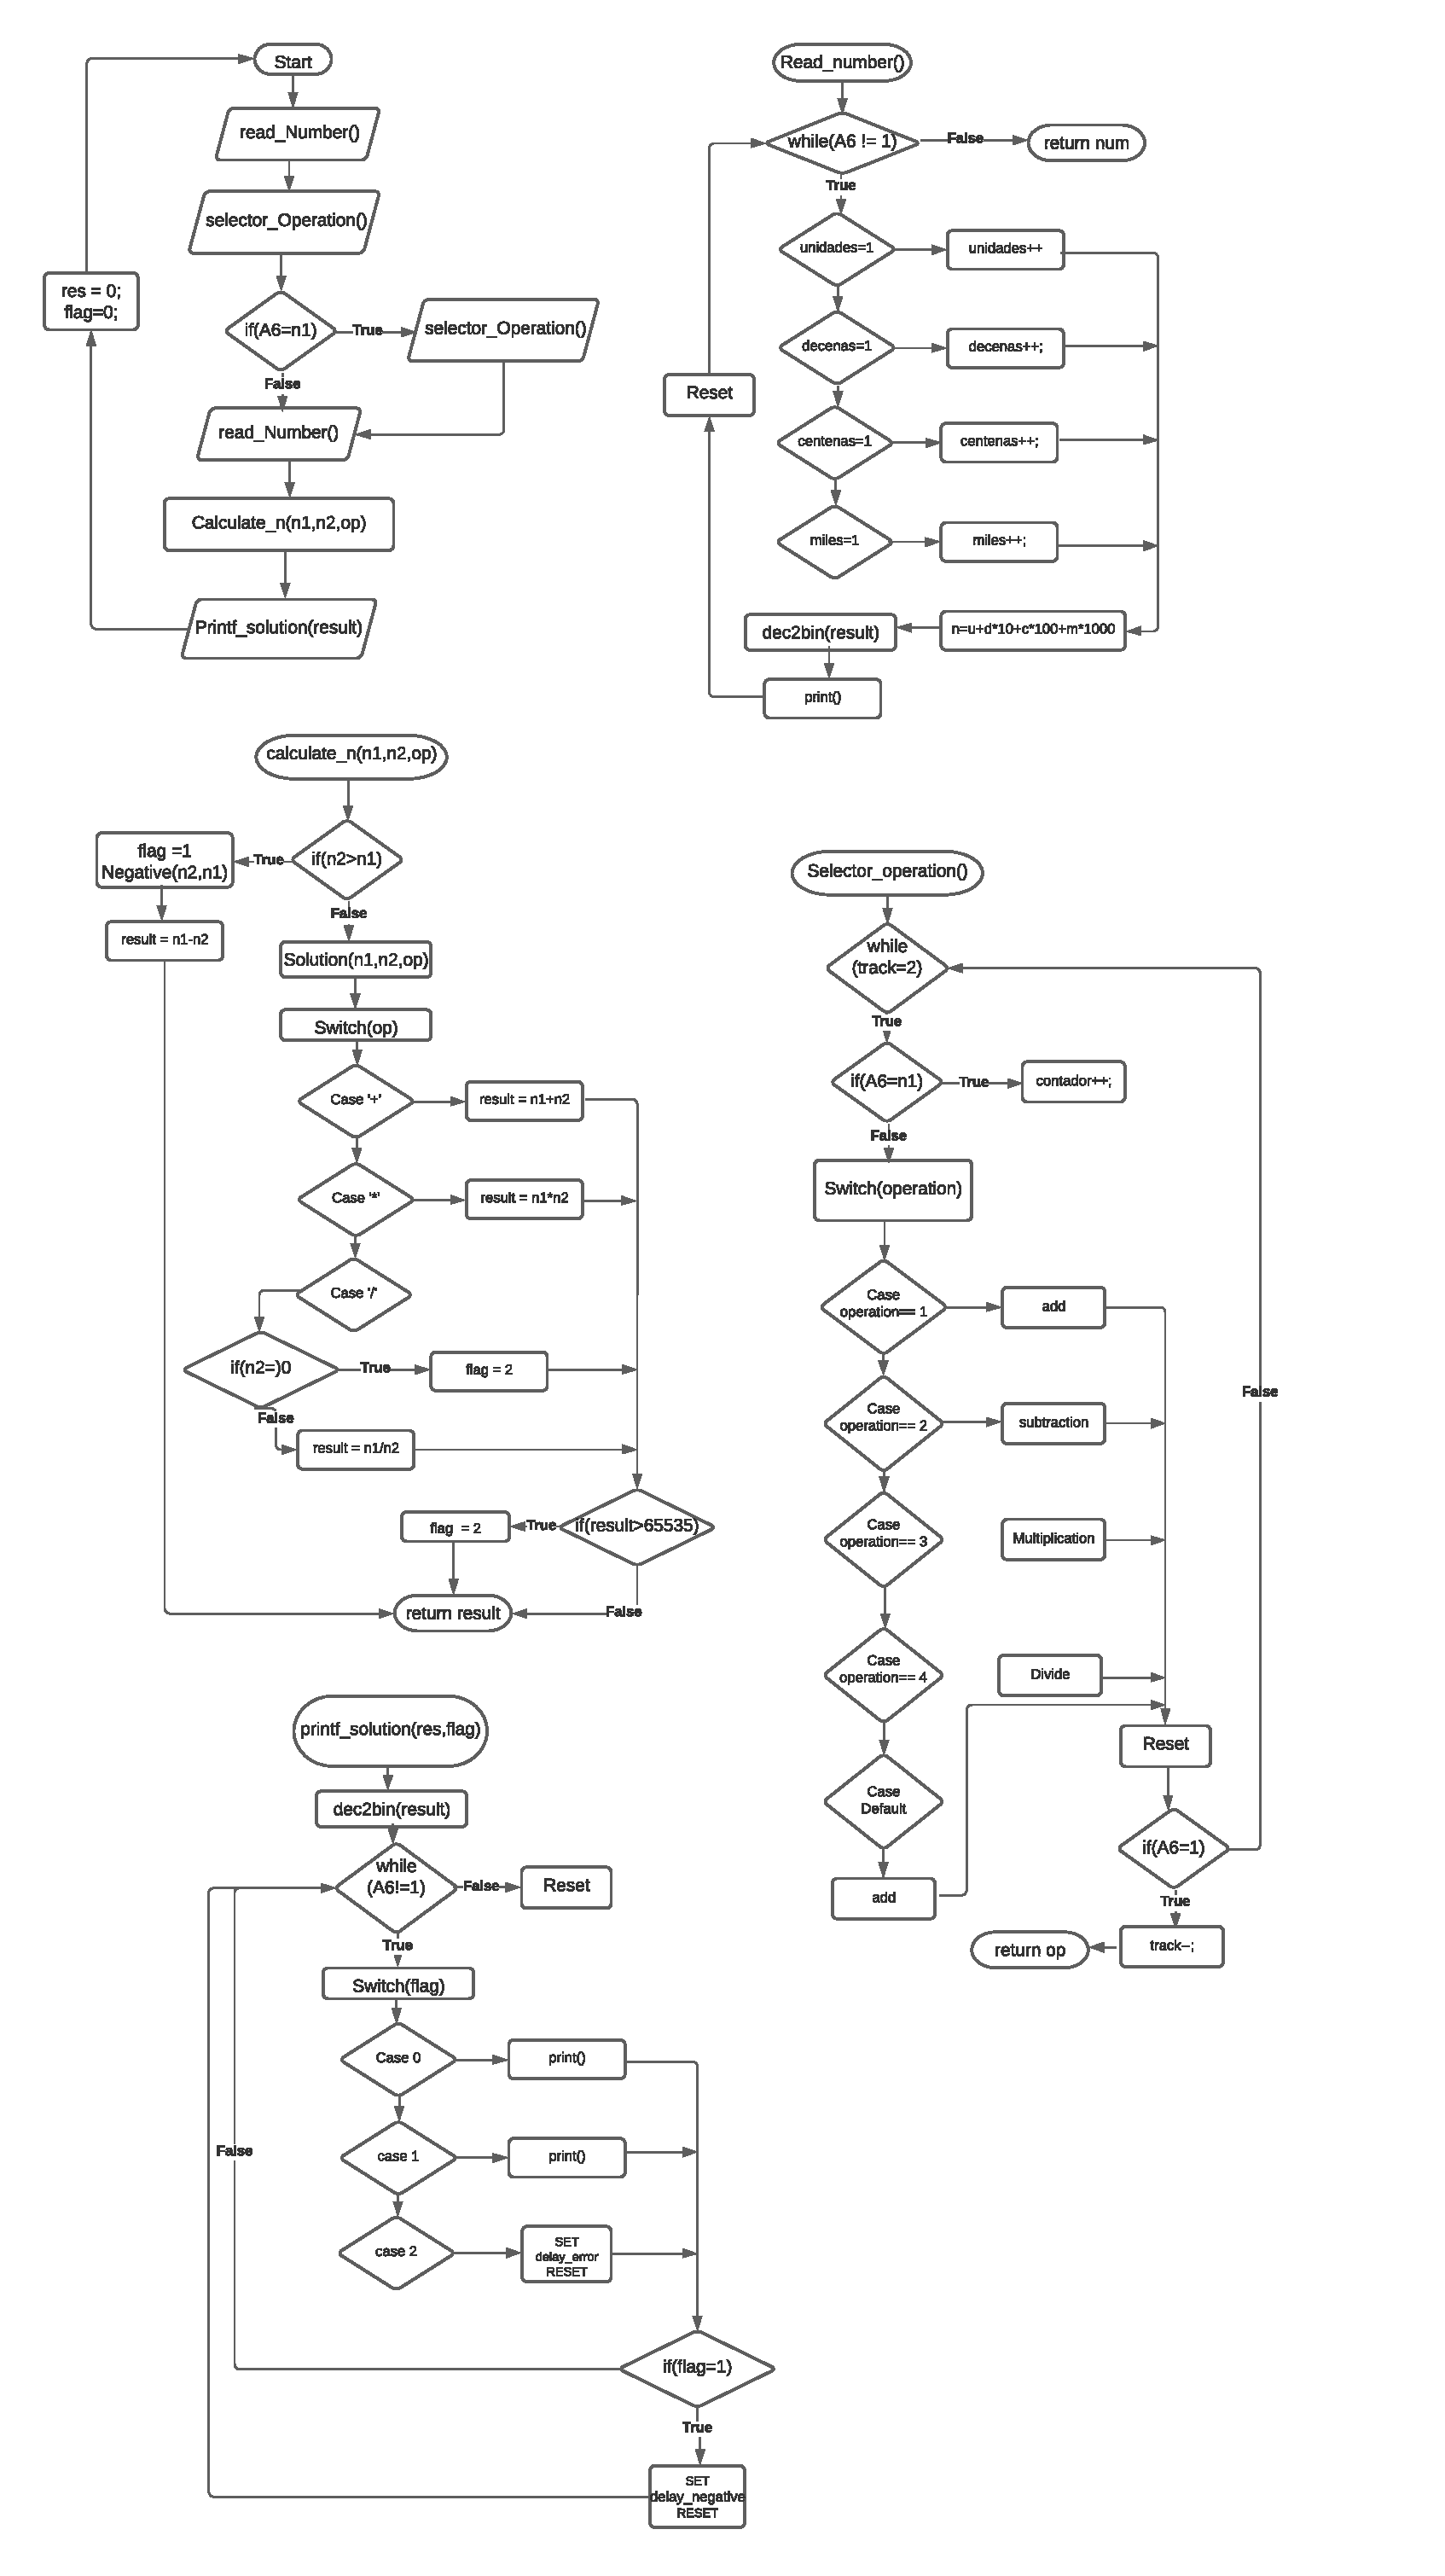
\includepdf[]{Anexos/Calculator.pdf}
\end{document}


